\section{VC Dimension}

\subsection{part a}
VC dimension of H is 3.

It is trivial to show that there exists one or two points on the plane that can be shattered by H. We now show that H is able to shatter 3 points which implies that the VC dimension of H is at least 3.

Select three points with coordinates A(1,1), B(-1,1) and C(-1, -1). There are 8 possible combinations in terms of labels. We claim that H is able to classify all the combinations.

The origin and radius choices are listed as follows to classify each combination. The order of the terms in each line is: label of point A, label of point B, label of point C, origin, radius.
\begin{itemize}
\item +, +, +, (0,0), 2
\item -, -, -, (0,0), 0.5
\item +, -, -, (1,0), 1
\item +, -, +, (1,-1), 2
\item -, +, -, (-1,1), 1
\item -, +, +, (-1,0), 1
\item -, -, +, (-1,-1), 0.5
\item +, +, -, (0,1), 1
\end{itemize}

So we proved that the VC dimension of H is at least 3.

Next, we show that H is not able to shatter any four points on the plane which means that the VC dimension of H is less than 4.

There are two possible situations when randomly choose four points:
\begin{itemize}
\item Four points form a convex hull. This situation cannot be classified by any hypotheses in H when the opposing points with the largest distance both have positive labels and the other two have negative labels.
\item Three points form a convex hull and one point is internal. This situation cannot be classified when the first three points (on the convex hull) have positive label and the fourth point has negative label.
\end{itemize}

Therefore, we proved that the VC dimension of H is 3.

%%%%%%%%%%%%%%%%%%%%%%%%%%%%%%%%%%%%%%%%%%
\subsection{part b}
VC dimension of H is 2k.

We start with the base case with one point $x_1$ on the real line. It is easy to see that we are able to shatter this point no matter it has a positive label (choose $a_1<x_1<b_1$ or a negative label (choose $b_1<x_1<a_2$).

After observing the cases with two points and three points, we see that the most complicated case, which is also the hardest case, to classify is when neighboring points have opposite labels. For example, the most complicated case of four points is when $x_1$ and $x_3$ have positive labels and $x_2$ and $x_4$ have negative labels. The reason that it is the hardest case to classify is because each of these four points need to be placed or assigned to a disjoint interval. This leads to the requirement of four disjoint intervals. As long as we have enough intervals, at least four intervals, to cope this situation, the points are shattered. Figure \ref{fig:p1} gives an illustration of this situation.

\begin{figure}[!htb]
\centering
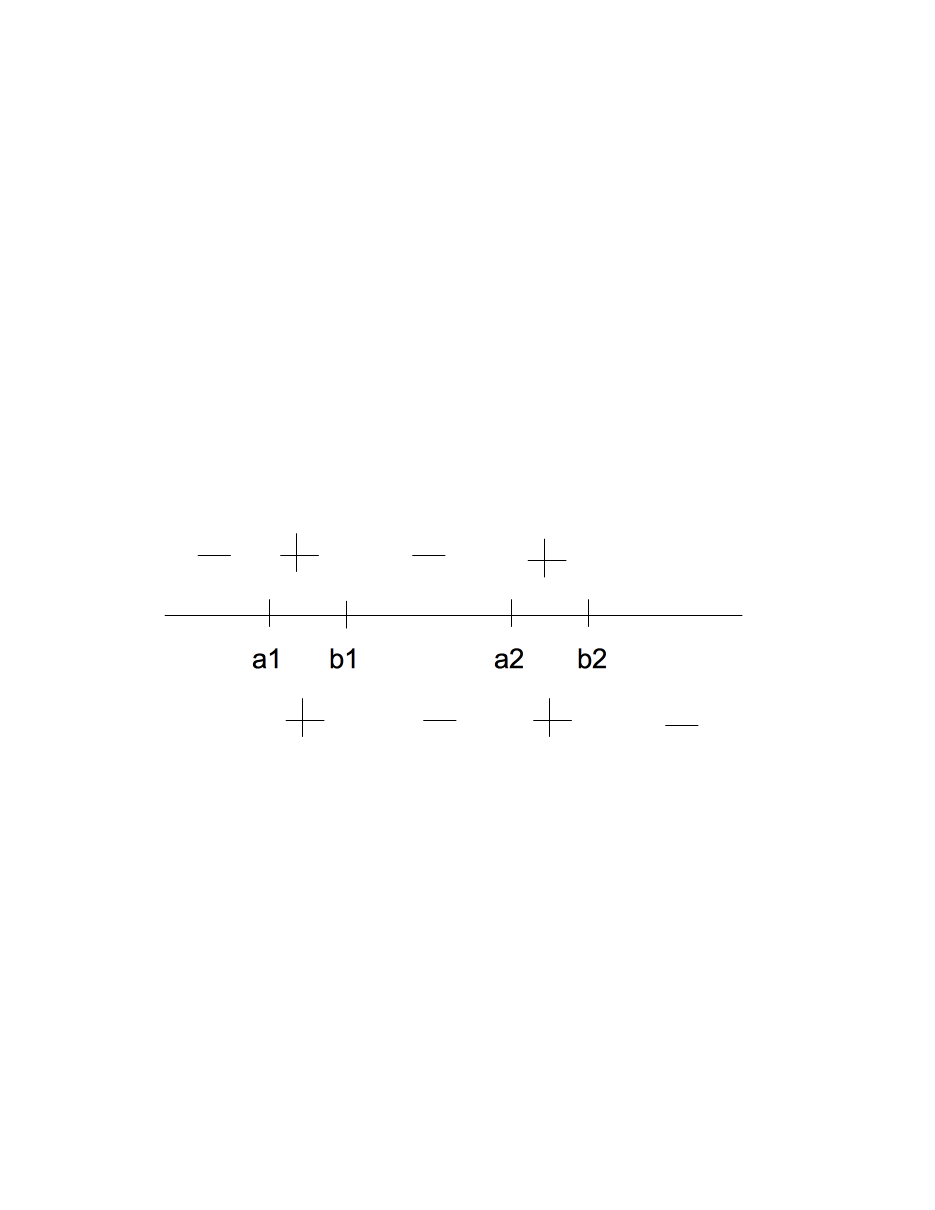
\includegraphics[trim=0 300 0 330, clip = true, scale=.5]{p1.png}
\caption{Four points with neghboring potins have opposite labels.}
\label{fig:p1}
\end{figure}

Note that with 4 parameters we have 5 intervals on the real line, however, the maximum number of points that could be shattered with these 4 parameters is only 4 which is described in Figure \ref{fig:p1}.

Now, we generalize the situation to 2k points on the real line. There are k disjoint intervals within which points are labeled as positive and another k+1 disjoint intervals within which points are negative. The largest number of points that can be shattered is 2k since we are able to assign at most 2k points with neighboring points have opposite labels into 2k intervals.

So far, we showed that the VC dimension of H is at least 2k.

Next, we show that H cannot shatter 2k+1 points. Again, consider the most complicated situation with the leftmost point with a positive label. Since the leftmost point must fall in the region where $x_{leftmost}>a_1$, there is no way any hypothesis from H can classify the right most point which has a positive label.

Therefore, we proved that the VC dimension of H is 2k.







